\section{Anomaly detection in timeseries of networks}
\label{sec:ch9:anomaly}

In many situations, you might have sequences of networks that study the same fundamental underlying system, but differ in one key respect: the networks are measured at different points in time. Data that studies the same objects measured over different points in time is known as \textit{longitudinal}. Let's begin by starting this section off with Example \ref{box:ch9:anomaly:ex} to see longitudinal data with networks.

\begin{floatingbox}[h]\caption{Case Study: brain networks of sea slugs}
\label{box:ch9:anomaly:ex}
There is a particular type of sea slug which has gills on the outside of its body. These gills are extremely sensitive, and are essential for the survival of the slug in the wild. When the gills sense any stimulus, the slug will reflexively withdraw the gills into the body. When the gill response is repeatedly triggered without a negative effect on the slug, the gill response diminishes, which has been connected to a form of memory \cite{Carew1971Aug,Kandel2001Nov}. However, when an electrical shock is administered, such as by a sting ray (a natural predator of the slug), the gill response returns. Experiments on these sea slugs were foundational to uncovering a physiological basis of memory in the brain, and led to the Nobel Prize in Physiology or Medicine in $2000$.

Say you’re a researcher studying these sea slugs, and you have a bunch of brain networks of the same slug. We can define each node as a single neuron, and edges denote connections between neurons. Each of the brain networks that you have were taken at different time point in which the slug's gill response was stimulated: some are before the slug learns not to withdraw its gills, some are after learning, and some are after an electrical shock is administered. You hypothesize that the brain networks will differ in the slug after learning and after the administration of an electrical shock. Given the network data you have, how do you figure out which timepoints these are?
\end{floatingbox}

The broader class of problems this question addresses is called \textit{anomaly detection}. The idea, is that you have a bunch of snapshots of a network that is evolving over time. Although the nodes are the same, the edges are being measured at different timepoints. Your goal is to figure out which time points correspond to the most change, either in the entire network or in particular groups of nodes. You can think of a network as ``anomalous'' with respect to time if some potentially small group of nodes within the network concurrently changes behavior at some point in time compared to the recent past, while the remaining nodes continue with whatever noisy, normal behavior they had.

In particular, what we would really like to do is separate the signal from the noise. All of the nodes in the network are likely changing a bit over time, since there is some variability intrinsic in the system (the measurement process itself is noisy, which we discussed in Section \ref{sec:ch1:challenges}). Random noise might just dictate that some edges spuriously exist or do not exist at different timepoints. We want to figure out if there are timepoints where the change is not just measurement variation: we are trying to figure out a point in time where the probability distribution that the network itself is generated from changes.

We will imagine our sea slug brain is measured at $T=12$ points in time where the sea slug is squirted with water on its gills. Each of our networks will have $90$ nodes representing neurons, in one of three communities of nodes representing the sensory neurons (responsible for reflexes), the hippocampus (responsible for memory), and the occipital lobe (responsible for sight). A pair of nodes are connected if they are working together at that timepoint.

For the first $6$ timepoints, when the sea slug is squirted, the network has a strong affinity structure, where within-community connections existing with probability $0.4$, and between-community connections existing with probability $0.05$. When the gills are squirted, the slug contracts them to protect them from damage.

After the $6^{th}$ timepoint, the slug has finally caught on. When the slug begins to learn that the water squirts are harmless, its memory center (the hippocampus) begins to modulate its response to the squirt bottle (controlled by the sensory neurons), and the slug reflexes its gills less.  The brain network of the slug sees a degree augmentation for its nodes during this time, via a degree-correction factor $\vec\theta$. By this point, the sea slug avoids reflexing its gills all together, once it has learned that the splashes are harmless.

Finally, after the $9^{th}$ timepoint, an electrical shock is administered to the slug prior to the water squirt, and the slug ``forgets'' that the water squirt itself is harmless. At this time point, the sea slug returns to its original brain patterns. We can generate the networks like this:

\begin{lstlisting}[style=python]
import numpy as np
from graspologic.simulations import sbm
from graphbook_code import dcsbm

# the block matrix for the neurons before learning
B0 = 0.05*np.ones((3, 3))
np.fill_diagonal(B0, 0.4)

nk = 30
ns = np.repeat(nk, 3)

theta = np.tile(np.linspace(np.sqrt(2), np.sqrt(2) - 1, nk), 3)
print(theta)
zs = np.repeat([1,2,3], 30)

T = 12
networks = np.array([sbm(ns, B0) if (t < 6 or t > 9) else dcsbm(zs, theta, B0) for t in range(T)])
\end{lstlisting}

The simulated networks are illustrated in Figure \ref{fig:ch9:anomaly:ex}. Notice that after learning in Figure \ref{fig:ch9:anomaly:ex}(B), the network does not look appreciably different; the only real change we can visually discern is that the nodes in the lower half of each community appear to have more edges than the nodes in the upper half of each community. However, this difference is not immediately apparent just through visualization alone. Next, after an electric shock is administered in Figure \ref{fig:ch9:anomaly:ex}(C), this pattern appears to return to the baseline response from Figure \ref{fig:ch9:anomaly:ex}(A).

\begin{figure}[h]
    \centering
    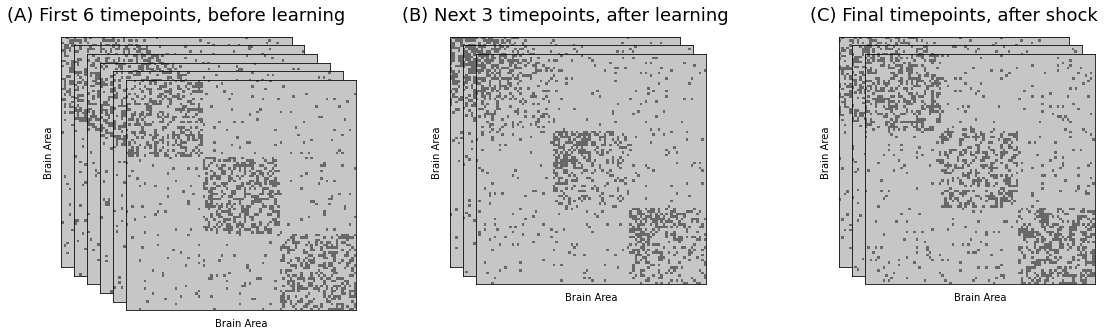
\includegraphics[width=\linewidth]{applications/ch9/Images/anom_ex.png}
    \caption[Longitudinal network data]{\textbf{(A)} the simulated networks, before learning, \textbf{(B)} the simulated networks, after learning, and \textbf{(C)} the simulated networks, after an electric shock is administered.}
    \label{fig:ch9:anomaly:ex}
\end{figure}

\subsection{Detecting anomalies using network models}

So, our goal is to detect which timepoints the network is changing by the most at. In words, if the network $A^{(t)}$ is a realization of a $\mathbf A^{(t)}$ random network that has probability matrix $P^{(t)}$, we want to identify the timepoints $t$ where $P^{(t)} \neq P^{(t - 1)}$, or that the probability matrix changes for the current timepoint compared to the preceding timepoint.

This gives us the hypotheses:
\begin{align*}
    H_0^{(t)} : P^{(t)} = P^{(t - 1)} \text{ against }H_A^{(t)} : P^{(t)} \neq P^{(t - 1)}
\end{align*}
for every timepoint $t$. 

Notice that if there were only two timepoints in total and $T = 2$, that this is equivalent to the hypotheses in Equation \eqref{eqn:ch8:twosample:2shypo_prob} from Section \ref{sec:ch8:twosample}. 

By the same logic that we gave there, a sensible approach to performing this test would be to instead test:
\begin{align*}
    H_0^{(t)} : X^{(t)} = WX^{(t - 1)} \text{ for some rotation matrix }W \\
    H_A^{(t)}: X^{(t)} \neq WX^{(t - 1)} \text{ for any rotation matrix }W,
\end{align*}
which is a latent position test from Section \ref{sec:ch8:twosample:lpt}. To do this in practice, we found in Equation \eqref{eqn:ch8:twosample:opp} that we could estimate the best possible rotation of the second estimated latent position matrix onto the first by solving the Orthogonal Procrustes Problem. We perform these latent position tests for all timepoints from $2$ to $T$, by sequentially comparing a given timepoint $t$ to the previous timepoint $t - 1$.

Each of these $T - 1$ tests gives us an estimated $p$-value, $\hat p^{(t)}$, which is estimated using the same parametric bootstrap procedure as previously described \cite{Tang2017Apr}. We consider a timepoint \textit{anomalous} if $\hat p^{(t)} \leq \alpha$, where as usual, we typically use $\alpha = 0.05$.

\paragraph*{The multiple comparisons problem, revisited}

In the case where there is no longitudinal effect (and the underlying networks are identical across time), we can again run into the \textit{multiple comparisons problem} from Section \ref{sec:ch8:twosamplesbm}. To recap, in statistical inference, if the null hypothesis is true (and there is no effect), we would expect about $\alpha$ fraction of tests run to have a $p$-value $\leq \alpha$. 

As we discussed previously, even though the error rate for an individual test at a given timepoint was $\alpha$, the Familywise Error Rate (FWER) for making an error for any of the $(T - 1)$ tests is $(T - 1)\alpha$. This means that if we have $T$ timepoints and there is no longitudinal effect (the null hypothesis is true), we would expect about $(T - 1)\alpha$ to falsely reject the null hypothesis in favor of the alternative hypothesis.

A fundamental solution to this issue was to use Bonferroni-Holm adjustment \cite{Holm1979}, which we will use here too.

\subsection{Applying anomaly detection to simulated networks}

Let's see how we can implement these ideas for anomaly testing. We obtain estimated $p$-values by using the latent position test from Section \ref{sec:ch8:twosample:lpt}:

\begin{lstlisting}[style=python]
from graspologic.inference import latent_position_test
import warnings

warnings.filterwarnings('ignore')
pvalues = [latent_position_test(networks[t + 1], networks[t], n_components=3, n_bootstraps=1000, workers=-1)[1] for t in range(T-1)]
\end{lstlisting}

next, we adjust for multiple comparisons, using the \texttt{multipletests()} function from \texttt{statsmodels}:

\begin{lstlisting}[style=python]
from statsmodels.stats.multitest import multipletests

alpha = 0.05
_, adj_pvals, _, _ = multipletests(pvalues, alpha=alpha, method="holm")
\end{lstlisting}

\begin{figure}
    \centering
    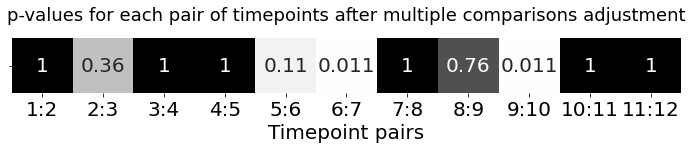
\includegraphics[width=\linewidth]{applications/ch9/Images/anom_pvals.png}
    \caption[Anomaly detection $p$-values]{The $p$-values from the latent position test for each pair of adjacent timepoints in the longitudinal sequence of networks.}
    \label{fig:ch9:anomaly:pvals}
\end{figure}
The resulting adjusted $p$-values are shown in Figure \ref{fig:ch9:anomaly:pvals}. Recall that timepoints $7$ through $9$ are the timepoints where the slug has ``learned'' that the water squirts are harmless. Therefore, for all pairs of timepoints from $1$ to $6$, $7$ to $9$, and $10$ to $12$, we should not be able to identify any difference. However, from $6$ to $7$ (when the slug learned) and from $9$ to $10$ (when the slug was shocked, and un-learned) we should be able to discern a difference. For these comparisons, the $p$-values (after adjustment) are below our detection threshold of $\alpha = 0.05$, indicating that we have evidence to reject the null hypothesis, and we find that the networks are different.